%_____________________________________________________________________________
%
%STRUTTURA RELAZIONE:
%
%istituto
%scopo -DONE
%introduzione teorica
%strumentazione  -DONE
%procedimento     
%dati sperimentali con tab
%elaborazione dati = calcoli teorici
%conclusione = confronto risultati teorici con dati sperimentali
%
%_____________________________________________________________________________

%NOTA UTILE: se in un testo bisogna inserire qualche dato numerico in riga, senza
%dover ricorrere a \begin{equation}, basta includere cio' che serve dentro a $....$
%esempio: $10k\Omega$ per inserire il dato in Ohm, poichè alcuni caratteri non vengono presi se stanno fuori da un'equazione


\documentclass{article}
\usepackage{amsmath}
\usepackage{setspace}
\usepackage{anysize}
\usepackage{geometry}
\usepackage{graphicx}
\graphicspath{ {./images/} }
%c'è 1 inch di margine a destra e sinistra
%\geometry{margin = 1.25 in}

\title{\huge \textbf{Relazione prima esperienza di laboratorio Fisica 2}}
\author{Gruppo A15: Armani Stefano, Cappellaro Nicola, Pasquato Leonardo}
\date{10-10-2022}
\vspace{0,25cm}
\setlength{\parindent}{0cm}
\vspace{0,25cm}


\begin{document}
    %print sezione titolo
    \maketitle
    \rule{\linewidth}{0.1mm}

    %scopo  Stefano
    \section{Scopo dell'esperienza}
    Lo scopo della nostra prima esperienza in laboratiorio è stato
    quella di familiarizzare con gli strumenti del laboratorio di elettronica
    che andremo a usare anche nelle esperienze future, principalmente con il
    generatore da banco e il multimetro e altri componenti elettrici,
    nel nostro caso i resistori.
    Grazie a questi strumenti andremo a misurare e verificare con dati reali
    alcune misure di tensione e il teorema di Millman.\par

    
    
        
    %introduzione teorica   Nicola
    \section{Cenni teorici}
    In questa prima esperienza utilizziamo e verificheremo la legge di Ohm utilizzando i resistori, mentre nel secondo esperimento
    verifichiamo il teorema di Millman per le reti elettriche. \par
    Ricordiamo:
    \begin{itemize}
        \item Legge di Ohm $V = R \cdot I$
        \item Legge di Kirchhoff delle correnti $\sum_{e = 1}^{n} i_e = \sum_{u = 1}^{m} i_u $
        \item Legge di Kirchhoff delle tensioni $\sum_{k = 1}^{n} V_k = 0 $
        \item Teorema di Millman $V_0 = \frac{\sum_{k = 1}^{n} \frac{V_k}{R_k} }{\sum_{k = 1}^{n} \frac{1}{R_k} }$
    \end{itemize}
    I circuiti realizzati sono di tipo lineare a tempo invariante e li chiameremo d'ora in poi (LTI)
    
    
    %elenco strumentazione
    \section{Strumentazione}
    \begin{itemize}
        \item Breadboard con annessi morsetti serrafilo;
        \item Cavi con connettori "a banana";
        \item Resistori di varie misure ($1k\Omega$, $10k\Omega$, $100k\Omega$, $1M\Omega$, $10M\Omega$);
        \item Connettori da banco (Jumper);
        \item Multimetro;
        \item Alimentatore da banco (generatore di corrente e tensione).
    \end{itemize}

    %descrizione esperimento    Leonardo
    \section{Esperimento}
    Una volta messo a disposizione il kit contenente la strumentazione indicata al punto $3$, %fai link
    si è esposto il primo esercizio riguardante un semplice \textbf{partitore di tensione}.
    Il partitore di tensione è un circuito LTI di prim'ordine come in figura, composto da:
    \begin{itemize}
        \item Generatore di tensione;
        \item 2 resistenze in serie;
        \item un multimetro collegato in parallelo alla seconda resistenza
    \end{itemize}
    %INSERISCI FIGURA DELLO SCHEMATICO DEL CIRCUITO + FOTO REALE
    %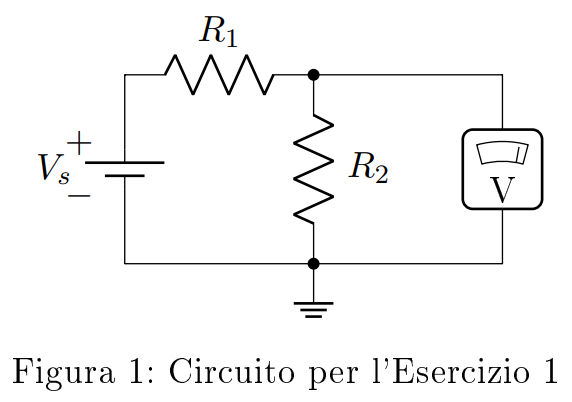
\includegraphics{circuito1.png}
    %provo a mettere la foto
    Si è successivamente replicato lo stesso circuito su una \textbf{Breadboard} utilizzando due resistori da
    $1k\Omega$, connettori da banco per collegare la Breadboard ai morsetti serrafilo connessi al generatore
    tramite \textbf{connettori a banana}. \par
    Successivamente sono stati accesi il multimetro e il generatore e, per primo step, sono stati impostati i limiti di corrente e tensione massima
    erogabile dal generatore, rispettivamente a $6mA$ e $6V$.\par
    A questo punto è stato possibile attivare il generatore affinchè nel circuito venisse mantenuta la tensione voluta e,
    grazie al multimetro impostato in modo tale da fungere da voltmetro, è stato possibile ottenere la tensione di lato della
    seconda resistenza in serie. La tensione di lato ottenuta è stata pari a $3.020V$.
    Successivamente, è stato ripetuto lo stesso esperimento utilizzando diversi resistori, ottenendo risultati leggermente diversi.\par
    I risultati più discostati dai precedenti sono sicuramente stati rilevati nelle ultime due misurazioni in cui sono state utilizzati
    resistori con resistenze ben più alte rispetto alle precedenti.\par
    \par
    %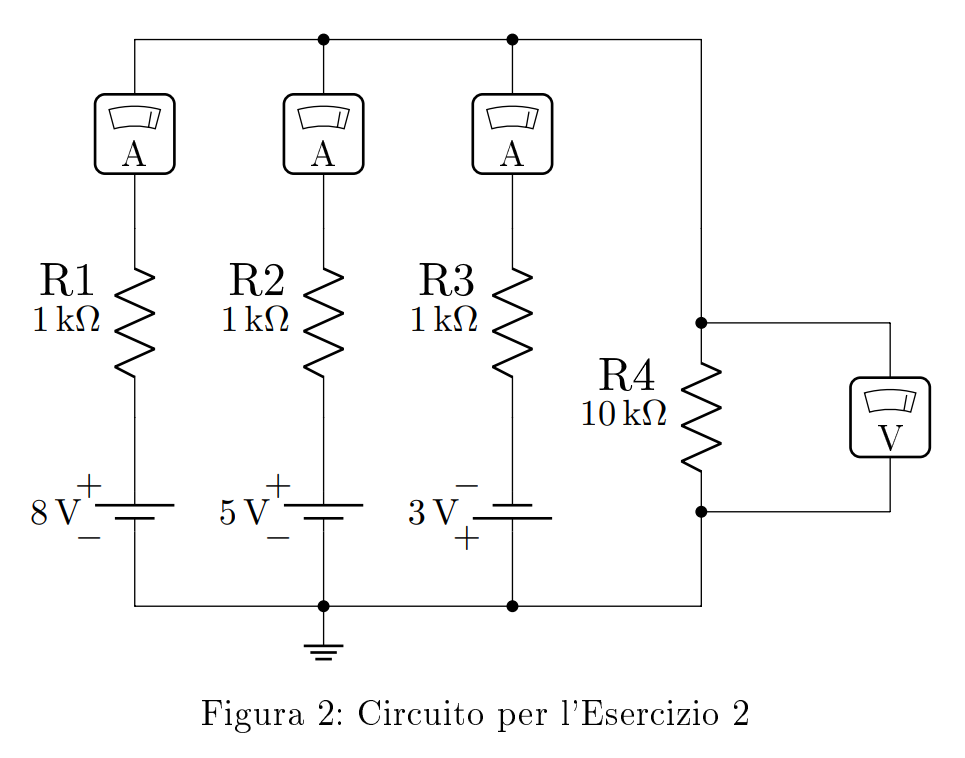
\includegraphics{circuito2.png}
    Nella seconda parte di questa esperienza di laboratorio è stato illustrato dal punto di vista teorico
    un teorema derivante dalle leggi di \textbf{Kirchhoff}, ossia il teorema di \textbf{Jacob Millman}.
    Dopo un'illustrazione teorica, è stato esposto un secondo esercizio in cui si può verificare sperimentalmente il teorema di Millman:
    %foto esercizio e foto circuito
    Una volta costruito l'esercizio sono state ripetute 3 misurazioni da parte del multimetro impostato come 
    amperometro, in modo tale da poter misurare sperimentalmente le correnti uscenti da tutte le resistenze.\par
    Ottenuti i valori delle correnti, è stato valutato la tensione di lato sulla resistenza da $10k\Omega$, come in figura:
    Questa misurazione coincide sperimentalmente con la tensione calcolata tramite il teorema di Millman.\par

    %risulati sperimentali

    \newpage

    \section{Dati sperimentali}
    \begin{center}
        Primo esperimento: \par
    \begin{tabular}{|c|c|c|c|}
        \hline
        \textit{Test} & \textit{Primo resistore} & \textit{Secondo resistore} & \textit{Tensione di lato} \\
        \hline
        Test 1 & $R_1 =1k\Omega$ & $R_2=1k\Omega$ & $V=3,020V$\\
        \hline
        Test 2 & $R_1 =1k\Omega$ & $R_2=500\Omega$ & $V=2,011V$\\
        \hline
        Test 3 & $R_1 =10k\Omega$ & $R_2=10k\Omega$ & $V=3,007V$\\
        \hline
        Test 4 & $R_1 =100k\Omega$ & $R_2=100k\Omega$ & $V=2,987V$\\
        \hline
        Test 5 & $R_1 =1M\Omega$ & $R_2=1\Omega$ & $V=2,857$\\
        \hline
        Test 6 & $R_1 =10\Omega$ & $R_2=10\Omega$ & $V=1,836$\\
        \hline
    
    \end{tabular}
    \end{center}
    
    \begin{center}
        Secondo esperimento: \par
    \begin{tabular}{|c|c|c|}
        \hline
        \textit{Ramo cortocircuitato} & \textit{Tensione} & \textit{Corrente} \\
        \hline
        Primo ramo & $V_1 = 8V$ & $I_1 = 4,782 mA$\\
        \hline
        Secondo ramo & $V_2 = 5V$ & $I_2 = 1,695 mA$\\
        \hline
        Terzo ramo & $V_3 = -3V$ & $I_3 = 6,276 mA$\\
        \hline
        & V di lato & $3,198 V$\\
        \hline
    
    \end{tabular}
    \end{center}


    
    %elaborazione dati  Leonardo
    \section{Elaborazione dati}
    Primo esperimento, $V_s = 6V$:
    \begin{align*}
        I_s = \frac{V_s}{R_{eq}}  \hspace{2cm}   & v_{R_2} = \frac{V_s}{V_{eq}} \cdot R_2  \hspace{2cm} &  V_{eq} = R_1 + R_2 \\
        & V_{Test1} = \frac{6V}{1k\Omega + 1k\Omega} \cdot 1k\Omega = 3V \\
        & V_{Test2} = \frac{6V}{1k\Omega + 500\Omega} \cdot 500\Omega = 2V \\
        & V_{Test3} = \frac{6V}{10k\Omega + 10k\Omega} \cdot 10k\Omega = 3V \\
        & V_{Test4} = \frac{6V}{100k\Omega + 100k\Omega} \cdot 100k\Omega = 3V \\
        & V_{Test5} = \frac{6V}{1M\Omega + 1M\Omega} \cdot 1M\Omega = 3V \\
        & V_{Test6} = \frac{6V}{10M\Omega + 10M\Omega} \cdot 1M\Omega = 3V \\
    \end{align*}

    Secondo esperimento:
    \begin{align*}
       & V = \frac{\frac{V_1}{R_1} + \frac{V_2}{R_2} + \frac{V_3}{R_3}}{\frac{1}{R_1} + \frac{1}{R_2} + \frac{1}{R_3} + \frac{1}{R_4}}\\
       & V = \frac{\frac{8V}{1k\Omega} + \frac{5V}{1k\Omega} + \frac{-3V}{1k\Omega}}{\frac{1}{1k\Omega} + \frac{1}{1k\Omega} + \frac{1}{1k\Omega} + \frac{1}{10k\Omega}} = 3,226V
    \end{align*}
    


    %conclusione
    \section{Conclusione}
    Nel primo esperimento abbiamo ottenuto dei valori di tensione molto vicini a quelli teorici con i resistori inferiori ad $1M\Omega$.
    Mentre abbiamo ottenuto dei valori di tensione inferiori a quelli attesi quando abbiamo usato i resistori da $1M\Omega$ ed $10M\Omega$
    Questo perché anche il voltmetro è un componente con una sua resistenza interna, quindi aggiungendolo al circuito
    viene attraversato da corrente ed è come se ci fosse un ulteriore resistenza in parallelo.

    D'altra parte nel secondo esperimento abbiamo visto che il teorema di Millman è verificato e siamo riusciti a trovare la tensione
    di lato applicando la formula e misurando effettivamente le singole correnti 


\end{document}